\documentclass[twoside]{book}

% Packages required by doxygen
\usepackage{fixltx2e}
\usepackage{calc}
\usepackage{doxygen}
\usepackage[export]{adjustbox} % also loads graphicx
\usepackage{graphicx}
\usepackage[utf8]{inputenc}
\usepackage{makeidx}
\usepackage{multicol}
\usepackage{multirow}
\PassOptionsToPackage{warn}{textcomp}
\usepackage{textcomp}
\usepackage[nointegrals]{wasysym}
\usepackage[table]{xcolor}

% Font selection
\usepackage[T1]{fontenc}
\usepackage[scaled=.90]{helvet}
\usepackage{courier}
\usepackage{amssymb}
\usepackage{sectsty}
\renewcommand{\familydefault}{\sfdefault}
\allsectionsfont{%
  \fontseries{bc}\selectfont%
  \color{darkgray}%
}
\renewcommand{\DoxyLabelFont}{%
  \fontseries{bc}\selectfont%
  \color{darkgray}%
}
\newcommand{\+}{\discretionary{\mbox{\scriptsize$\hookleftarrow$}}{}{}}

% Page & text layout
\usepackage{geometry}
\geometry{%
  a4paper,%
  top=2.5cm,%
  bottom=2.5cm,%
  left=2.5cm,%
  right=2.5cm%
}
\tolerance=750
\hfuzz=15pt
\hbadness=750
\setlength{\emergencystretch}{15pt}
\setlength{\parindent}{0cm}
\setlength{\parskip}{3ex plus 2ex minus 2ex}
\makeatletter
\renewcommand{\paragraph}{%
  \@startsection{paragraph}{4}{0ex}{-1.0ex}{1.0ex}{%
    \normalfont\normalsize\bfseries\SS@parafont%
  }%
}
\renewcommand{\subparagraph}{%
  \@startsection{subparagraph}{5}{0ex}{-1.0ex}{1.0ex}{%
    \normalfont\normalsize\bfseries\SS@subparafont%
  }%
}
\makeatother

% Headers & footers
\usepackage{fancyhdr}
\pagestyle{fancyplain}
\fancyhead[LE]{\fancyplain{}{\bfseries\thepage}}
\fancyhead[CE]{\fancyplain{}{}}
\fancyhead[RE]{\fancyplain{}{\bfseries\leftmark}}
\fancyhead[LO]{\fancyplain{}{\bfseries\rightmark}}
\fancyhead[CO]{\fancyplain{}{}}
\fancyhead[RO]{\fancyplain{}{\bfseries\thepage}}
\fancyfoot[LE]{\fancyplain{}{}}
\fancyfoot[CE]{\fancyplain{}{}}
\fancyfoot[RE]{\fancyplain{}{\bfseries\scriptsize Generated by Doxygen }}
\fancyfoot[LO]{\fancyplain{}{\bfseries\scriptsize Generated by Doxygen }}
\fancyfoot[CO]{\fancyplain{}{}}
\fancyfoot[RO]{\fancyplain{}{}}
\renewcommand{\footrulewidth}{0.4pt}
\renewcommand{\chaptermark}[1]{%
  \markboth{#1}{}%
}
\renewcommand{\sectionmark}[1]{%
  \markright{\thesection\ #1}%
}

% Indices & bibliography
\usepackage{natbib}
\usepackage[titles]{tocloft}
\setcounter{tocdepth}{3}
\setcounter{secnumdepth}{5}
\makeindex

% Hyperlinks (required, but should be loaded last)
\usepackage{ifpdf}
\ifpdf
  \usepackage[pdftex,pagebackref=true]{hyperref}
\else
  \usepackage[ps2pdf,pagebackref=true]{hyperref}
\fi
\hypersetup{%
  colorlinks=true,%
  linkcolor=blue,%
  citecolor=blue,%
  unicode%
}

% Custom commands
\newcommand{\clearemptydoublepage}{%
  \newpage{\pagestyle{empty}\cleardoublepage}%
}

\usepackage{caption}
\captionsetup{labelsep=space,justification=centering,font={bf},singlelinecheck=off,skip=4pt,position=top}

%===== C O N T E N T S =====

\begin{document}

% Titlepage & ToC
\hypersetup{pageanchor=false,
             bookmarksnumbered=true,
             pdfencoding=unicode
            }
\pagenumbering{alph}
\begin{titlepage}
\vspace*{7cm}
\begin{center}%
{\Large Joint Level Control }\\
\vspace*{1cm}
{\large Generated by Doxygen 1.8.13}\\
\end{center}
\end{titlepage}
\clearemptydoublepage
\pagenumbering{roman}
\tableofcontents
\clearemptydoublepage
\pagenumbering{arabic}
\hypersetup{pageanchor=true}

%--- Begin generated contents ---
\chapter{Joint Level Control}
\label{index}\hypertarget{index}{}\hypertarget{index_intro}{}\section{Introduction}\label{index_intro}
This is the documentation for the Tri\+Ped Projects joint level controller. It implements the Hardware Interfaces required by \href{http://wiki.ros.org/ros_control}{\tt ros\+\_\+control} to interface the joint position and joint space trajectory controllers with the sensors and actuators. A Diagram of how this package interfaces with ros\+\_\+\+Control can be seen here\+:  The Naming conventions for each joint, motor, and sensor are specified in the \href{https://github.com/TriPed-Robot/Wiki/wiki/One-Legged-Sub-Robot}{\tt wiki} and can be seen down below\+:  \hypertarget{index_arch}{}\section{Hardware Interface Architecture}\label{index_arch}
Each Leg of the Tri\+Ped robot, is made up of two types of joints, extend joints and swing joints each requiring its own hardware interface. Since both types of joints share the same motor controller each hardware interface is designed as a class containing a motor class object and a sensor class object. The rotary\+\_\+encoder class is the sensor class used by the extend\+\_\+joint interface, while the hall\+\_\+sensor class is used by the swing\+\_\+joint\+\_\+interface. \hypertarget{index_content}{}\section{Structure of the Project}\label{index_content}
The Project is designed as \href{http://wiki.ros.org/Packages}{\tt R\+OS package} and is distributed into the following directories\+:


\begin{DoxyItemize}
\item config
\end{DoxyItemize}

docs
\begin{DoxyItemize}
\item include
\item launch
\item src 
\end{DoxyItemize}\hypertarget{index_config_dir}{}\subsection{config}\label{index_config_dir}
The project is designed to be flexible in regards to different configurations, for this reason, hardware addresses, and other device-\/specific parameters are always read in from config files. This folder contains all necessary config files for the joint controllers. On startup of the joint controllers, these config files are first set as \href{http://wiki.ros.org/Parameter%20Server}{\tt R\+OS parameters} and then subsequently read out by the approprate \href{http://wiki.ros.org/Nodes}{\tt R\+OS nodes}. \hypertarget{index_docs_dir}{}\subsection{docs}\label{index_docs_dir}
The docs folder houses the Doxygen documentation from which this page is generated. It is not necessary for the proper functioning of this package. \hypertarget{index_include_dir}{}\subsection{include}\label{index_include_dir}
The include directory contains the c++ header files of the package. This special directory is necessary for the \href{http://wiki.ros.org/catkin/commands/catkin_make}{\tt catkin\+\_\+make} to find the files. The name of the include directory is specified in the C\+Make\+List file. \hypertarget{index_launch_dir}{}\subsection{launch}\label{index_launch_dir}
The launch directory contains all \href{http://wiki.ros.org/roslaunch}{\tt R\+OS launch files} of the package. It contains the following files

\tabulinesep=1mm
\begin{longtabu} spread 0pt [c]{*{2}{|X[-1]}|}
\hline
\rowcolor{\tableheadbgcolor}\textbf{ launch file name }&\textbf{ purpose  }\\\cline{1-2}
\endfirsthead
\hline
\endfoot
\hline
\rowcolor{\tableheadbgcolor}\textbf{ launch file name }&\textbf{ purpose  }\\\cline{1-2}
\endhead
hall\+\_\+sensor\+\_\+test &Testing the Hall Sensors \\\cline{1-2}
motor &Testing the \hyperlink{classMotor}{Motor} \\\cline{1-2}
joint\+\_\+level\+\_\+control &Start the Joint controllers \\\cline{1-2}
\end{longtabu}
Each launchfile also loads the parameters of the config directory. \hypertarget{index_src_dir}{}\subsection{src}\label{index_src_dir}
This directory contains the source code of the package.\hypertarget{index_bbb_setup}{}\section{Beaglebone Black Setup}\label{index_bbb_setup}
In order to use the joint controller the I/O of the Beaglebone black has to be set up according to the \href{https://github.com/TriPed-Robot/Wiki/wiki/Beaglebone-Setup}{\tt beaglebone setup guide} Afterwards the sensors and actuators have to be connected according to the \href{https://github.com/TriPed-Robot/Wiki/wiki/Wiring-diagram}{\tt wiring diagram}. \hypertarget{index_getting_started}{}\section{Getting Started}\label{index_getting_started}
This section details the steps neccesairy to install the joint\+\_\+level\+\_\+control package and use it to controll the joints of the Tri\+Ped.\hypertarget{index_install}{}\subsection{Installing the Package}\label{index_install}
Since the project is a ros package, it has to be placed inside the src directory of a \href{http://wiki.ros.org/catkin}{\tt catkin\+\_\+ws}, and installed with {\ttfamily catkin\+\_\+make}\+:

\begin{DoxyVerb}$ cd catkin_ws/src
$ git clone https://github.com/TriPed-Robot/joint_level_control
$ cd ..
$ catkin_make
$ source devel/setup.sh
\end{DoxyVerb}


To verify that the package was installed one can call


\begin{DoxyCode}
$ rospack joint\_level\_control
\end{DoxyCode}


Which should provide informations about the package \hypertarget{index_usage}{}\subsection{Using the Package}\label{index_usage}

\chapter{Beaglebone Black Setup}
\label{bbb_setup}
\Hypertarget{bbb_setup}
In order to use the joint controller the I/O of the Beaglebone black has to be set up according to the \href{https://github.com/TriPed-Robot/Wiki/wiki/Beaglebone-Setup}{\tt beaglebone setup guide} Afterwards the sensors and actuators have to be connected according to the \href{https://github.com/TriPed-Robot/Wiki/wiki/Wiring-diagram}{\tt wiring diagram}. 
\chapter{R\+E\+A\+D\+ME}
\label{md__home_jan_TriPed_Robot_joint_level_control_README}
\Hypertarget{md__home_jan_TriPed_Robot_joint_level_control_README}
This is repository contains the joint controller for the Tri\+Ped robot. It implements the Hardware Interfaces required by \href{http://wiki.ros.org/ros_control}{\tt ros\+\_\+control} to interface the joint position and joint space trajectory controllers with the sensors and actuators. A Diagram of how this package interfaces with ros\+\_\+\+Control can be seen here\+:  The Documentation of this repository can be seen \href{https://triped-robot.github.io/joint_level_control/html/index.html}{\tt here}. 
\chapter{Hierarchical Index}
\section{Class Hierarchy}
This inheritance list is sorted roughly, but not completely, alphabetically\+:\begin{DoxyCompactList}
\item \contentsline{section}{Control\+Response}{\pageref{structControlResponse}}{}
\item \contentsline{section}{Hall\+Sensor}{\pageref{classHallSensor}}{}
\item \contentsline{section}{Message}{\pageref{structMessage}}{}
\item \contentsline{section}{Message\+Builder}{\pageref{classMessageBuilder}}{}
\begin{DoxyCompactList}
\item \contentsline{section}{Current\+Control}{\pageref{classCurrentControl}}{}
\item \contentsline{section}{Ping\+Message}{\pageref{classPingMessage}}{}
\item \contentsline{section}{Scan\+Message}{\pageref{classScanMessage}}{}
\end{DoxyCompactList}
\item \contentsline{section}{Message\+Parser}{\pageref{classMessageParser}}{}
\item \contentsline{section}{Motor}{\pageref{classMotor}}{}
\item \contentsline{section}{Multiple\+Controller\+Parser}{\pageref{classMultipleControllerParser}}{}
\item Robot\+HW\begin{DoxyCompactList}
\item \contentsline{section}{Extend\+Joint}{\pageref{classExtendJoint}}{}
\item \contentsline{section}{Swing\+Joint}{\pageref{classSwingJoint}}{}
\end{DoxyCompactList}
\item \contentsline{section}{Rotary\+Encoder}{\pageref{classRotaryEncoder}}{}
\item \contentsline{section}{Scan\+Response}{\pageref{structScanResponse}}{}
\end{DoxyCompactList}

\chapter{Class Index}
\section{Class List}
Here are the classes, structs, unions and interfaces with brief descriptions\+:\begin{DoxyCompactList}
\item\contentsline{section}{\hyperlink{structcan__frame}{can\+\_\+frame} \\*Stub to simplify development on non Linux Systems }{\pageref{structcan__frame}}{}
\item\contentsline{section}{\hyperlink{structControlResponse}{Control\+Response} }{\pageref{structControlResponse}}{}
\item\contentsline{section}{\hyperlink{classCurrentControl}{Current\+Control} \\*This subclass generates Current-\/\+Control Messages which allow to control the motor via a current limit }{\pageref{classCurrentControl}}{}
\item\contentsline{section}{\hyperlink{classExtendJoint}{Extend\+Joint} }{\pageref{classExtendJoint}}{}
\item\contentsline{section}{\hyperlink{classHallSensor}{Hall\+Sensor} }{\pageref{classHallSensor}}{}
\item\contentsline{section}{\hyperlink{structMessage}{Message} }{\pageref{structMessage}}{}
\item\contentsline{section}{\hyperlink{classMessageBuilder}{Message\+Builder} \\*This class and its subclasses handle the creation of the C\+A\+N-\/\+Frames needed to control the Hacker Herkules 5 B\+L\+DC }{\pageref{classMessageBuilder}}{}
\item\contentsline{section}{\hyperlink{classMessageParser}{Message\+Parser} }{\pageref{classMessageParser}}{}
\item\contentsline{section}{\hyperlink{classMotor}{Motor} }{\pageref{classMotor}}{}
\item\contentsline{section}{\hyperlink{classMultipleControllerParser}{Multiple\+Controller\+Parser} }{\pageref{classMultipleControllerParser}}{}
\item\contentsline{section}{\hyperlink{classPingMessage}{Ping\+Message} \\*This subclass generates a Ping-\/\+Message so that one can verify if a controller with an known address is active }{\pageref{classPingMessage}}{}
\item\contentsline{section}{\hyperlink{classRotaryEncoder}{Rotary\+Encoder} }{\pageref{classRotaryEncoder}}{}
\item\contentsline{section}{\hyperlink{classScanMessage}{Scan\+Message} \\*This subclass generates a Scan-\/\+Message so that new Controllers on the C\+A\+N-\/\+Bus can be found }{\pageref{classScanMessage}}{}
\item\contentsline{section}{\hyperlink{structScanResponse}{Scan\+Response} }{\pageref{structScanResponse}}{}
\item\contentsline{section}{\hyperlink{classSwingJoint}{Swing\+Joint} }{\pageref{classSwingJoint}}{}
\end{DoxyCompactList}

\chapter{Class Documentation}
\hypertarget{structControlResponse}{}\section{Control\+Response Struct Reference}
\label{structControlResponse}\index{Control\+Response@{Control\+Response}}
\subsection*{Public Attributes}
\begin{DoxyCompactItemize}
\item 
\mbox{\Hypertarget{structControlResponse_a186d016869eb2ce90a2436cfb4d04e8c}\label{structControlResponse_a186d016869eb2ce90a2436cfb4d04e8c}} 
int16\+\_\+t {\bfseries battery\+\_\+current}
\item 
\mbox{\Hypertarget{structControlResponse_afa59d2c9e3d8dda3ebdcd7c5e17fa5f2}\label{structControlResponse_afa59d2c9e3d8dda3ebdcd7c5e17fa5f2}} 
int16\+\_\+t {\bfseries motor\+\_\+current}
\item 
\mbox{\Hypertarget{structControlResponse_a3d47770ef278ec131d29a7409b46a4e2}\label{structControlResponse_a3d47770ef278ec131d29a7409b46a4e2}} 
uint16\+\_\+t {\bfseries battery\+\_\+voltage}
\item 
\mbox{\Hypertarget{structControlResponse_af6848f07b4e4ae2e6cd49d90983b229a}\label{structControlResponse_af6848f07b4e4ae2e6cd49d90983b229a}} 
uint16\+\_\+t {\bfseries reserved\+\_\+data}
\item 
\mbox{\Hypertarget{structControlResponse_aebf2539ed484813d25e925a198c7849a}\label{structControlResponse_aebf2539ed484813d25e925a198c7849a}} 
uint16\+\_\+t {\bfseries ppm\+\_\+adc}
\item 
\mbox{\Hypertarget{structControlResponse_a137abb16394ba1cda8bf7de163776311}\label{structControlResponse_a137abb16394ba1cda8bf7de163776311}} 
int16\+\_\+t {\bfseries motor\+\_\+temperature}
\item 
\mbox{\Hypertarget{structControlResponse_a20ee2b4e5fd6a8328ce713c6d9b681e0}\label{structControlResponse_a20ee2b4e5fd6a8328ce713c6d9b681e0}} 
int16\+\_\+t {\bfseries erpm}
\item 
\mbox{\Hypertarget{structControlResponse_a6245c488d394e709d19e6d69fc9aece6}\label{structControlResponse_a6245c488d394e709d19e6d69fc9aece6}} 
int16\+\_\+t {\bfseries rpm}
\item 
\mbox{\Hypertarget{structControlResponse_abcbc48206cf93810547848b6042b39f0}\label{structControlResponse_abcbc48206cf93810547848b6042b39f0}} 
uint16\+\_\+t {\bfseries pwm\+\_\+frequency}
\item 
\mbox{\Hypertarget{structControlResponse_abeb5c1b5e5fed33dcfb6595b06ad8d1b}\label{structControlResponse_abeb5c1b5e5fed33dcfb6595b06ad8d1b}} 
int16\+\_\+t {\bfseries pwm\+\_\+duty}
\item 
\mbox{\Hypertarget{structControlResponse_ad11ecc5814970e9b7a3f0d9471d07ae1}\label{structControlResponse_ad11ecc5814970e9b7a3f0d9471d07ae1}} 
int16\+\_\+t {\bfseries pcb\+\_\+temperature}
\item 
\mbox{\Hypertarget{structControlResponse_af726a4b6a342d214b606a048ed070989}\label{structControlResponse_af726a4b6a342d214b606a048ed070989}} 
state\+\_\+t {\bfseries state}
\item 
\mbox{\Hypertarget{structControlResponse_a73672473e86060a346b0d55d3c1ac62d}\label{structControlResponse_a73672473e86060a346b0d55d3c1ac62d}} 
fault\+\_\+t {\bfseries fault}
\end{DoxyCompactItemize}


The documentation for this struct was generated from the following file\+:\begin{DoxyCompactItemize}
\item 
/sd/triped\+\_\+app/catkin\+\_\+workspace/src/joint\+\_\+level\+\_\+control/include/joint\+\_\+level\+\_\+control/motor/response\+\_\+messages.\+h\end{DoxyCompactItemize}

\hypertarget{classCurrentControl}{}\section{Current\+Control Class Reference}
\label{classCurrentControl}\index{Current\+Control@{Current\+Control}}


This subclass generates Current-\/\+Control Messages which allow to control the motor via a current limit.  




{\ttfamily \#include $<$message\+\_\+builder.\+h$>$}



Inheritance diagram for Current\+Control\+:\nopagebreak
\begin{figure}[H]
\begin{center}
\leavevmode
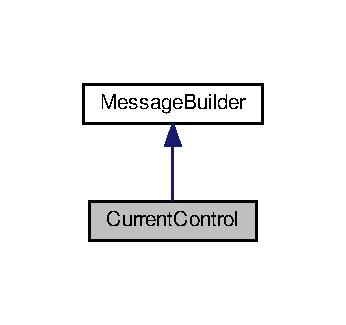
\includegraphics[width=166pt]{classCurrentControl__inherit__graph}
\end{center}
\end{figure}


Collaboration diagram for Current\+Control\+:\nopagebreak
\begin{figure}[H]
\begin{center}
\leavevmode
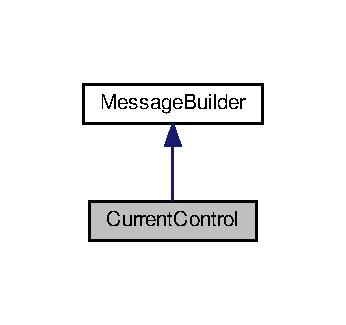
\includegraphics[width=166pt]{classCurrentControl__coll__graph}
\end{center}
\end{figure}
\subsection*{Public Member Functions}
\begin{DoxyCompactItemize}
\item 
\hyperlink{classCurrentControl_a3e56845d95613d4c55d7b8dde7cc8300}{Current\+Control} (uint8\+\_\+t address)
\item 
void \hyperlink{classCurrentControl_a5096783dd03da0895cd352fc9977736d}{set\+Current} (int32\+\_\+t current)
\end{DoxyCompactItemize}
\subsection*{Additional Inherited Members}


\subsection{Detailed Description}
This subclass generates Current-\/\+Control Messages which allow to control the motor via a current limit. 

\subsection{Constructor \& Destructor Documentation}
\index{Current\+Control@{Current\+Control}!Current\+Control@{Current\+Control}}
\index{Current\+Control@{Current\+Control}!Current\+Control@{Current\+Control}}
\subsubsection[{\texorpdfstring{Current\+Control(uint8\+\_\+t address)}{CurrentControl(uint8_t address)}}]{\setlength{\rightskip}{0pt plus 5cm}Current\+Control\+::\+Current\+Control (
\begin{DoxyParamCaption}
\item[{uint8\+\_\+t}]{address}
\end{DoxyParamCaption}
)}\hypertarget{classCurrentControl_a3e56845d95613d4c55d7b8dde7cc8300}{}\label{classCurrentControl_a3e56845d95613d4c55d7b8dde7cc8300}
Constructor of the \hyperlink{classCurrentControl}{Current\+Control} Class 
\begin{DoxyParams}{Parameters}
{\em address} & C\+A\+N-\/\+ID of the B\+L\+DC which is controlled by this class instance. \\
\hline
\end{DoxyParams}


\subsection{Member Function Documentation}
\index{Current\+Control@{Current\+Control}!set\+Current@{set\+Current}}
\index{set\+Current@{set\+Current}!Current\+Control@{Current\+Control}}
\subsubsection[{\texorpdfstring{set\+Current(int32\+\_\+t current)}{setCurrent(int32_t current)}}]{\setlength{\rightskip}{0pt plus 5cm}void Current\+Control\+::set\+Current (
\begin{DoxyParamCaption}
\item[{int32\+\_\+t}]{current}
\end{DoxyParamCaption}
)}\hypertarget{classCurrentControl_a5096783dd03da0895cd352fc9977736d}{}\label{classCurrentControl_a5096783dd03da0895cd352fc9977736d}
Sets the current of this class instance. 
\begin{DoxyParams}{Parameters}
{\em current} & The current which should be set. N\+O\+TE\+: Current is set in 0.\+1A increments. set\+Current(1) will set the B\+L\+DC to 0.\+1 A \\
\hline
\end{DoxyParams}


The documentation for this class was generated from the following files\+:\begin{DoxyCompactItemize}
\item 
message\+\_\+builder.\+h\item 
current\+\_\+control.\+cpp\end{DoxyCompactItemize}

\hypertarget{classExtendJoint}{}\section{Extend\+Joint Class Reference}
\label{classExtendJoint}\index{Extend\+Joint@{Extend\+Joint}}


Inheritance diagram for Extend\+Joint\+:
\nopagebreak
\begin{figure}[H]
\begin{center}
\leavevmode
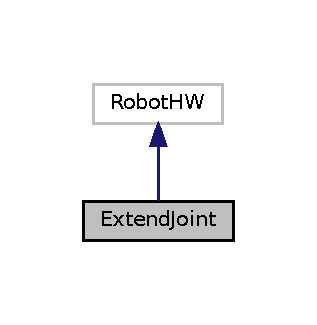
\includegraphics[width=152pt]{classExtendJoint__inherit__graph}
\end{center}
\end{figure}


Collaboration diagram for Extend\+Joint\+:
\nopagebreak
\begin{figure}[H]
\begin{center}
\leavevmode
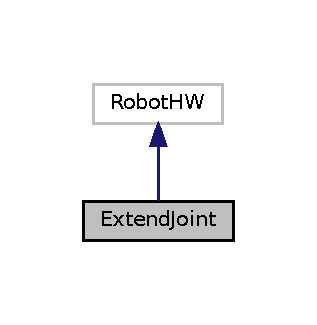
\includegraphics[width=152pt]{classExtendJoint__coll__graph}
\end{center}
\end{figure}
\subsection*{Public Member Functions}
\begin{DoxyCompactItemize}
\item 
\mbox{\Hypertarget{classExtendJoint_a115a7b5763d4496e9c365614241b2351}\label{classExtendJoint_a115a7b5763d4496e9c365614241b2351}} 
{\bfseries Extend\+Joint} (const std\+::string \&joint\+\_\+name, const std\+::string \&spi\+\_\+device, uint8\+\_\+t spi\+\_\+cs\+\_\+id, uint8\+\_\+t spi\+\_\+mode, uint8\+\_\+t spi\+\_\+bits, uint32\+\_\+t spi\+\_\+speed, uint16\+\_\+t spi\+\_\+delay, const std\+::string \&can\+\_\+name, uint8\+\_\+t can\+\_\+id)
\item 
\mbox{\Hypertarget{classExtendJoint_a703426ab8a4047bb7a6087ffff734b5d}\label{classExtendJoint_a703426ab8a4047bb7a6087ffff734b5d}} 
void {\bfseries read} ()
\item 
\mbox{\Hypertarget{classExtendJoint_aaaddc50f230254a001ce8b3f56064371}\label{classExtendJoint_aaaddc50f230254a001ce8b3f56064371}} 
void {\bfseries write} ()
\end{DoxyCompactItemize}


The documentation for this class was generated from the following files\+:\begin{DoxyCompactItemize}
\item 
/sd/triped\+\_\+app/catkin\+\_\+workspace/src/joint\+\_\+level\+\_\+control/include/joint\+\_\+level\+\_\+control/joint/extend\+\_\+joint.\+h\item 
/sd/triped\+\_\+app/catkin\+\_\+workspace/src/joint\+\_\+level\+\_\+control/src/joint/extend\+\_\+joint.\+cpp\end{DoxyCompactItemize}

\hypertarget{classHallSensor}{}\section{Hall\+Sensor Class Reference}
\label{classHallSensor}\index{Hall\+Sensor@{Hall\+Sensor}}


This class abstracts the communication with the sensors measuring the state of the swingjoints.  




{\ttfamily \#include $<$hall\+\_\+sensor.\+h$>$}

\subsection*{Public Member Functions}
\begin{DoxyCompactItemize}
\item 
\hyperlink{classHallSensor_ac901b856eff0dffb4dfa5fdeaf888c4c}{Hall\+Sensor} (const std\+::string \&spi\+\_\+device, uint8\+\_\+t spi\+\_\+cs\+\_\+id, uint8\+\_\+t spi\+\_\+mode, uint8\+\_\+t spi\+\_\+bits, uint32\+\_\+t spi\+\_\+speed, uint16\+\_\+t spi\+\_\+delay, double zero\+\_\+point)
\begin{DoxyCompactList}\small\item\em Constructor of the \hyperlink{classHallSensor}{Hall\+Sensor} class. \end{DoxyCompactList}\item 
double \hyperlink{classHallSensor_a5eea1969e798bc786c5fa165aeb47c77}{get\+Value} ()
\item 
void \hyperlink{classHallSensor_ac97079734e670ba56401e6a8b37144e8}{set\+Zero\+Point} ()
\end{DoxyCompactItemize}


\subsection{Detailed Description}
This class abstracts the communication with the sensors measuring the state of the swingjoints. 

The left and right swingsensor, measure the position the swingjoints. They are implemented using As5047D Hall Sensors as well as magnets attached to the output lever of the motor assembly (pictured below).  The magnets are affixed using 3d printed caps, which offer no way to predetermine the magnetic field at a given angle. This means that the sensor output which is initially in counts has to be calibrated. This is done either during initialization using the zero\+\_\+point value or during runtime using the set\+Zero\+Point method.

After initialization the sensors produce values in the range of \mbox{[}-\/pi,pi\mbox{]}. A angle of zero is specified as the angle at which the position of the output lever is perpendicular to the two mounting brackets of the hall sensor Because these mounting brackets constrict the movement output lever the actually achievable range of motion is \mbox{[}-\/pi/2,pi/2\mbox{]}.

The embedded communication with the Sensor is done via S\+PI according to their datasheet. The connection of the sensor to the beaglebone can be seen in the s\href{https://github.com/TriPed-Robot/Wiki/wiki/Wiring-diagram}{\tt wiring diagram}. 

\subsection{Constructor \& Destructor Documentation}
\mbox{\Hypertarget{classHallSensor_ac901b856eff0dffb4dfa5fdeaf888c4c}\label{classHallSensor_ac901b856eff0dffb4dfa5fdeaf888c4c}} 
\index{Hall\+Sensor@{Hall\+Sensor}!Hall\+Sensor@{Hall\+Sensor}}
\index{Hall\+Sensor@{Hall\+Sensor}!Hall\+Sensor@{Hall\+Sensor}}
\subsubsection{\texorpdfstring{Hall\+Sensor()}{HallSensor()}}
{\footnotesize\ttfamily Hall\+Sensor\+::\+Hall\+Sensor (\begin{DoxyParamCaption}\item[{const std\+::string \&}]{spi\+\_\+device,  }\item[{uint8\+\_\+t}]{spi\+\_\+cs\+\_\+id,  }\item[{uint8\+\_\+t}]{spi\+\_\+mode,  }\item[{uint8\+\_\+t}]{spi\+\_\+bits,  }\item[{uint32\+\_\+t}]{spi\+\_\+speed,  }\item[{uint16\+\_\+t}]{spi\+\_\+delay,  }\item[{double}]{zero\+\_\+point }\end{DoxyParamCaption})}



Constructor of the \hyperlink{classHallSensor}{Hall\+Sensor} class. 


\begin{DoxyParams}{Parameters}
{\em S\+PI} & device, Chip select ID, mode, number of bits, communication speed and delay as well as the angle which is considered zero by the kinematics. \\
\hline
\end{DoxyParams}


\subsection{Member Function Documentation}
\mbox{\Hypertarget{classHallSensor_a5eea1969e798bc786c5fa165aeb47c77}\label{classHallSensor_a5eea1969e798bc786c5fa165aeb47c77}} 
\index{Hall\+Sensor@{Hall\+Sensor}!get\+Value@{get\+Value}}
\index{get\+Value@{get\+Value}!Hall\+Sensor@{Hall\+Sensor}}
\subsubsection{\texorpdfstring{get\+Value()}{getValue()}}
{\footnotesize\ttfamily double Hall\+Sensor\+::get\+Value (\begin{DoxyParamCaption}{ }\end{DoxyParamCaption})}

Reads the Angle of the \hyperlink{classHallSensor}{Hall\+Sensor} \mbox{\Hypertarget{classHallSensor_ac97079734e670ba56401e6a8b37144e8}\label{classHallSensor_ac97079734e670ba56401e6a8b37144e8}} 
\index{Hall\+Sensor@{Hall\+Sensor}!set\+Zero\+Point@{set\+Zero\+Point}}
\index{set\+Zero\+Point@{set\+Zero\+Point}!Hall\+Sensor@{Hall\+Sensor}}
\subsubsection{\texorpdfstring{set\+Zero\+Point()}{setZeroPoint()}}
{\footnotesize\ttfamily void Hall\+Sensor\+::set\+Zero\+Point (\begin{DoxyParamCaption}{ }\end{DoxyParamCaption})}

Sets the next Angle sent from the Sensor as new zeropoint for the angles. 

The documentation for this class was generated from the following files\+:\begin{DoxyCompactItemize}
\item 
hall\+\_\+sensor.\+h\item 
hall\+\_\+sensor.\+cpp\end{DoxyCompactItemize}

\hypertarget{structMessage}{}\section{Message Struct Reference}
\label{structMessage}\index{Message@{Message}}
\subsection*{Public Attributes}
\begin{DoxyCompactItemize}
\item 
uint8\+\_\+t {\bfseries can\+\_\+address}\hypertarget{structMessage_acc056126eaea6e24ec077efdb187c703}{}\label{structMessage_acc056126eaea6e24ec077efdb187c703}

\item 
uint8\+\_\+t $\ast$ {\bfseries data}\hypertarget{structMessage_a858e7641c732b295c70e6fdb8db0fac9}{}\label{structMessage_a858e7641c732b295c70e6fdb8db0fac9}

\item 
Message\+Type {\bfseries type}\hypertarget{structMessage_a6fc78df47d3755e088e7c658db565fc5}{}\label{structMessage_a6fc78df47d3755e088e7c658db565fc5}

\end{DoxyCompactItemize}


The documentation for this struct was generated from the following file\+:\begin{DoxyCompactItemize}
\item 
hacker\+\_\+const.\+h\end{DoxyCompactItemize}

\hypertarget{classMessageBuilder}{}\section{Message\+Builder Class Reference}
\label{classMessageBuilder}\index{Message\+Builder@{Message\+Builder}}


This class and its subclasses handle the creation of the C\+A\+N-\/\+Frames needed to control the Hacker Herkules 5 B\+L\+DC.  




{\ttfamily \#include $<$message\+\_\+builder.\+h$>$}



Inheritance diagram for Message\+Builder\+:\nopagebreak
\begin{figure}[H]
\begin{center}
\leavevmode
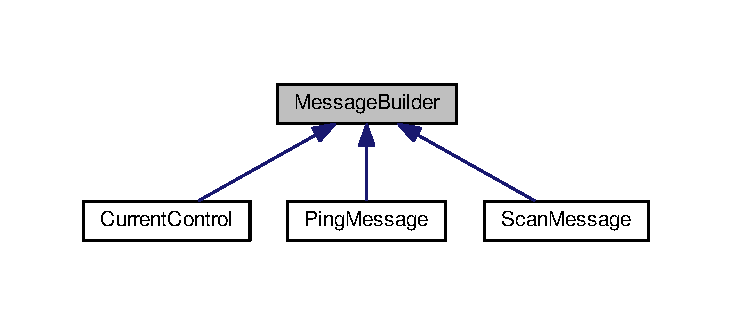
\includegraphics[width=350pt]{classMessageBuilder__inherit__graph}
\end{center}
\end{figure}
\subsection*{Public Member Functions}
\begin{DoxyCompactItemize}
\item 
\hyperlink{classMessageBuilder_a4323114db973ba35f2834b42d6b58aa7}{Message\+Builder} (uint8\+\_\+t address)
\begin{DoxyCompactList}\small\item\em Constructor of the \hyperlink{classMessageBuilder}{Message\+Builder} Class. \end{DoxyCompactList}\item 
can\+\_\+frame $\ast$ \hyperlink{classMessageBuilder_a588441e4327872e90c3442e1cecd50c3}{get\+Message} ()
\begin{DoxyCompactList}\small\item\em gets the generated Socket\+C\+A\+N-\/\+Frame for utilisation by the callee. \end{DoxyCompactList}\end{DoxyCompactItemize}
\subsection*{Protected Attributes}
\begin{DoxyCompactItemize}
\item 
\mbox{\Hypertarget{classMessageBuilder_abebf536b5645d60e62741e92a48f350a}\label{classMessageBuilder_abebf536b5645d60e62741e92a48f350a}} 
uint8\+\_\+t {\bfseries data} \mbox{[}8\mbox{]}
\item 
\mbox{\Hypertarget{classMessageBuilder_af8e2143bb0e870152961fe420d38596b}\label{classMessageBuilder_af8e2143bb0e870152961fe420d38596b}} 
uint8\+\_\+t {\bfseries can\+\_\+address}
\end{DoxyCompactItemize}


\subsection{Detailed Description}
This class and its subclasses handle the creation of the C\+A\+N-\/\+Frames needed to control the Hacker Herkules 5 B\+L\+DC. 

\subsection{Constructor \& Destructor Documentation}
\mbox{\Hypertarget{classMessageBuilder_a4323114db973ba35f2834b42d6b58aa7}\label{classMessageBuilder_a4323114db973ba35f2834b42d6b58aa7}} 
\index{Message\+Builder@{Message\+Builder}!Message\+Builder@{Message\+Builder}}
\index{Message\+Builder@{Message\+Builder}!Message\+Builder@{Message\+Builder}}
\subsubsection{\texorpdfstring{Message\+Builder()}{MessageBuilder()}}
{\footnotesize\ttfamily Message\+Builder\+::\+Message\+Builder (\begin{DoxyParamCaption}\item[{uint8\+\_\+t}]{address }\end{DoxyParamCaption})}



Constructor of the \hyperlink{classMessageBuilder}{Message\+Builder} Class. 


\begin{DoxyParams}{Parameters}
{\em address} & C\+A\+N-\/\+ID of the to-\/be controlled B\+L\+DC \\
\hline
\end{DoxyParams}


\subsection{Member Function Documentation}
\mbox{\Hypertarget{classMessageBuilder_a588441e4327872e90c3442e1cecd50c3}\label{classMessageBuilder_a588441e4327872e90c3442e1cecd50c3}} 
\index{Message\+Builder@{Message\+Builder}!get\+Message@{get\+Message}}
\index{get\+Message@{get\+Message}!Message\+Builder@{Message\+Builder}}
\subsubsection{\texorpdfstring{get\+Message()}{getMessage()}}
{\footnotesize\ttfamily can\+\_\+frame $\ast$ Message\+Builder\+::get\+Message (\begin{DoxyParamCaption}{ }\end{DoxyParamCaption})}



gets the generated Socket\+C\+A\+N-\/\+Frame for utilisation by the callee. 

\begin{DoxyReturn}{Returns}
can\+\_\+frame pointer for easy plug into write() 
\end{DoxyReturn}


The documentation for this class was generated from the following files\+:\begin{DoxyCompactItemize}
\item 
message\+\_\+builder.\+h\item 
message\+\_\+builder.\+cpp\end{DoxyCompactItemize}

\hypertarget{classMessageParser}{}\section{Message\+Parser Class Reference}
\label{classMessageParser}\index{Message\+Parser@{Message\+Parser}}
\subsection*{Public Member Functions}
\begin{DoxyCompactItemize}
\item 
\mbox{\Hypertarget{classMessageParser_abd504499821ba3076c3b5fcbe9709f59}\label{classMessageParser_abd504499821ba3076c3b5fcbe9709f59}} 
{\bfseries Message\+Parser} (uint8\+\_\+t can\+\_\+address)
\item 
\mbox{\Hypertarget{classMessageParser_a6106b34b152ee12e88e6a00cc88cb614}\label{classMessageParser_a6106b34b152ee12e88e6a00cc88cb614}} 
\hyperlink{structMessage}{message\+\_\+t} {\bfseries add\+Frame} (\hyperlink{structcan__frame}{can\+\_\+frame} frame)
\end{DoxyCompactItemize}


The documentation for this class was generated from the following files\+:\begin{DoxyCompactItemize}
\item 
/sd/triped\+\_\+app/catkin\+\_\+workspace/src/joint\+\_\+level\+\_\+control/include/joint\+\_\+level\+\_\+control/motor/message\+\_\+parser.\+h\item 
/sd/triped\+\_\+app/catkin\+\_\+workspace/src/joint\+\_\+level\+\_\+control/src/motor/message\+\_\+parser.\+cpp\end{DoxyCompactItemize}

\hypertarget{classMotor}{}\section{Motor Class Reference}
\label{classMotor}\index{Motor@{Motor}}
\subsection*{Public Member Functions}
\begin{DoxyCompactItemize}
\item 
\mbox{\Hypertarget{classMotor_a00bdaca43863fd9de6b48f5cf53bbfc3}\label{classMotor_a00bdaca43863fd9de6b48f5cf53bbfc3}} 
{\bfseries Motor} (const std\+::string \&can\+\_\+name, uint8\+\_\+t can\+\_\+id)
\item 
\mbox{\Hypertarget{classMotor_a7cb17a0f6e8aad3523348a1687bf549b}\label{classMotor_a7cb17a0f6e8aad3523348a1687bf549b}} 
void {\bfseries set\+Current} (int32\+\_\+t current)
\item 
\mbox{\Hypertarget{classMotor_a77185f4c17591bed876cbb3e5d8735f1}\label{classMotor_a77185f4c17591bed876cbb3e5d8735f1}} 
int {\bfseries write\+C\+AN} (\hyperlink{structcan__frame}{can\+\_\+frame} $\ast$frame)
\end{DoxyCompactItemize}


The documentation for this class was generated from the following files\+:\begin{DoxyCompactItemize}
\item 
/sd/triped\+\_\+app/catkin\+\_\+workspace/src/joint\+\_\+level\+\_\+control/include/joint\+\_\+level\+\_\+control/motor/motor.\+h\item 
/sd/triped\+\_\+app/catkin\+\_\+workspace/src/joint\+\_\+level\+\_\+control/src/motor/motor.\+cpp\end{DoxyCompactItemize}

\hypertarget{classMultipleControllerParser}{}\section{Multiple\+Controller\+Parser Class Reference}
\label{classMultipleControllerParser}\index{Multiple\+Controller\+Parser@{Multiple\+Controller\+Parser}}
\subsection*{Public Member Functions}
\begin{DoxyCompactItemize}
\item 
int {\bfseries add\+Controller} (uint8\+\_\+t can\+\_\+id)\hypertarget{classMultipleControllerParser_a9f7fc9bcef88ff36f78add7ee5e22fd3}{}\label{classMultipleControllerParser_a9f7fc9bcef88ff36f78add7ee5e22fd3}

\item 
\hyperlink{structMessage}{message\+\_\+t} {\bfseries handle\+Frame} (can\+\_\+frame frame)\hypertarget{classMultipleControllerParser_a8bef539882907a651c6ad1938da9f0e7}{}\label{classMultipleControllerParser_a8bef539882907a651c6ad1938da9f0e7}

\end{DoxyCompactItemize}


The documentation for this class was generated from the following files\+:\begin{DoxyCompactItemize}
\item 
multiple\+\_\+controller\+\_\+parser.\+h\item 
multiple\+\_\+controller\+\_\+parser.\+cpp\end{DoxyCompactItemize}

\hypertarget{classPingMessage}{}\section{Ping\+Message Class Reference}
\label{classPingMessage}\index{Ping\+Message@{Ping\+Message}}


This subclass generates a Ping-\/\+Message so that one can verify if a controller with an known address is active.  




{\ttfamily \#include $<$message\+\_\+builder.\+h$>$}



Inheritance diagram for Ping\+Message\+:\nopagebreak
\begin{figure}[H]
\begin{center}
\leavevmode
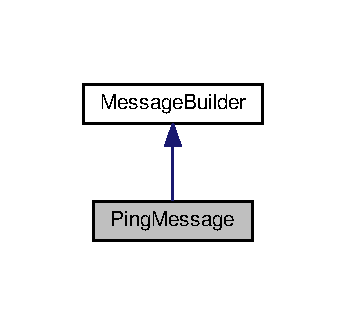
\includegraphics[width=174pt]{classPingMessage__inherit__graph}
\end{center}
\end{figure}


Collaboration diagram for Ping\+Message\+:\nopagebreak
\begin{figure}[H]
\begin{center}
\leavevmode
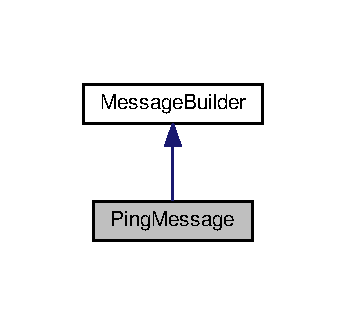
\includegraphics[width=174pt]{classPingMessage__coll__graph}
\end{center}
\end{figure}
\subsection*{Public Member Functions}
\begin{DoxyCompactItemize}
\item 
\hyperlink{classPingMessage_a67d49a8189b481cf1d39460a90ab5be7}{Ping\+Message} (uint8\+\_\+t address)
\end{DoxyCompactItemize}
\subsection*{Additional Inherited Members}


\subsection{Detailed Description}
This subclass generates a Ping-\/\+Message so that one can verify if a controller with an known address is active. 

\subsection{Constructor \& Destructor Documentation}
\mbox{\Hypertarget{classPingMessage_a67d49a8189b481cf1d39460a90ab5be7}\label{classPingMessage_a67d49a8189b481cf1d39460a90ab5be7}} 
\index{Ping\+Message@{Ping\+Message}!Ping\+Message@{Ping\+Message}}
\index{Ping\+Message@{Ping\+Message}!Ping\+Message@{Ping\+Message}}
\subsubsection{\texorpdfstring{Ping\+Message()}{PingMessage()}}
{\footnotesize\ttfamily Ping\+Message\+::\+Ping\+Message (\begin{DoxyParamCaption}\item[{uint8\+\_\+t}]{address }\end{DoxyParamCaption})}

Constructor of the \hyperlink{classPingMessage}{Ping\+Message} Class 
\begin{DoxyParams}{Parameters}
{\em address} & C\+A\+N-\/\+ID of the B\+L\+DC which should be pinged. \\
\hline
\end{DoxyParams}


The documentation for this class was generated from the following files\+:\begin{DoxyCompactItemize}
\item 
/sd/triped\+\_\+app/catkin\+\_\+workspace/src/joint\+\_\+level\+\_\+control/include/joint\+\_\+level\+\_\+control/motor/message\+\_\+builder.\+h\item 
/sd/triped\+\_\+app/catkin\+\_\+workspace/src/joint\+\_\+level\+\_\+control/src/motor/ping\+\_\+message.\+cpp\end{DoxyCompactItemize}

\hypertarget{classRotaryEncoder}{}\section{Rotary\+Encoder Class Reference}
\label{classRotaryEncoder}\index{Rotary\+Encoder@{Rotary\+Encoder}}


This class abstracts the communication with Sensors of the Extendjoints (currently a E6\+A2-\/C rotary encoder).  




{\ttfamily \#include $<$rotary\+\_\+encoder.\+h$>$}

\subsection*{Public Member Functions}
\begin{DoxyCompactItemize}
\item 
\hyperlink{classRotaryEncoder_ac57e2531f91e03b48bcc2b7e3f0edf62}{Rotary\+Encoder} (const std\+::string \&spi\+\_\+device, uint8\+\_\+t spi\+\_\+cs\+\_\+id, uint8\+\_\+t spi\+\_\+mode, uint8\+\_\+t spi\+\_\+bits, uint32\+\_\+t spi\+\_\+speed, uint16\+\_\+t spi\+\_\+delay)
\item 
double \hyperlink{classRotaryEncoder_adf89df36f38d0ee87b454f22c25a85f0}{get\+Value} ()
\end{DoxyCompactItemize}


\subsection{Detailed Description}
This class abstracts the communication with Sensors of the Extendjoints (currently a E6\+A2-\/C rotary encoder). 

This class abstracts the communication with the sensors measuring the state of the extendjoint.

The extendsensor measures the position of the extendjoint.\+This is is implemented using a omron E6\+A2-\/C rotary encoder which is connected to the drive shaft driven by the extendmotor and a photosensor (seen below)  The photosensor is needet since a rotary encoder does not measure absolute position. A splint affixed to the leg is able to trigger the photosensor thereby providing a absolute position feedback. There are multiple possible position of the splint, the current one can be seen below  The readout of rotary encoder and photosensor is abstracted by an arduino which sends the calibrated angle values over spi

It is important to note that the send angle is not the position of the driveshaft, but instead the state of the virtual extend joint. More information about this virtual joint can be found \href{https://github.com/TriPed-Robot/TriPed-Reference-Document}{\tt here}. 

\subsection{Constructor \& Destructor Documentation}
\mbox{\Hypertarget{classRotaryEncoder_ac57e2531f91e03b48bcc2b7e3f0edf62}\label{classRotaryEncoder_ac57e2531f91e03b48bcc2b7e3f0edf62}} 
\index{Rotary\+Encoder@{Rotary\+Encoder}!Rotary\+Encoder@{Rotary\+Encoder}}
\index{Rotary\+Encoder@{Rotary\+Encoder}!Rotary\+Encoder@{Rotary\+Encoder}}
\subsubsection{\texorpdfstring{Rotary\+Encoder()}{RotaryEncoder()}}
{\footnotesize\ttfamily Rotary\+Encoder\+::\+Rotary\+Encoder (\begin{DoxyParamCaption}\item[{const std\+::string \&}]{spi\+\_\+device,  }\item[{uint8\+\_\+t}]{spi\+\_\+cs\+\_\+id,  }\item[{uint8\+\_\+t}]{spi\+\_\+mode,  }\item[{uint8\+\_\+t}]{spi\+\_\+bits,  }\item[{uint32\+\_\+t}]{spi\+\_\+speed,  }\item[{uint16\+\_\+t}]{spi\+\_\+delay }\end{DoxyParamCaption})}

Constructor of the \hyperlink{classRotaryEncoder}{Rotary\+Encoder} class 
\begin{DoxyParams}{Parameters}
{\em S\+PI} & device, Chip select ID, mode, number of bits, communication speed and delay as well as the angle which is considered zero by the kinematics. \\
\hline
\end{DoxyParams}


\subsection{Member Function Documentation}
\mbox{\Hypertarget{classRotaryEncoder_adf89df36f38d0ee87b454f22c25a85f0}\label{classRotaryEncoder_adf89df36f38d0ee87b454f22c25a85f0}} 
\index{Rotary\+Encoder@{Rotary\+Encoder}!get\+Value@{get\+Value}}
\index{get\+Value@{get\+Value}!Rotary\+Encoder@{Rotary\+Encoder}}
\subsubsection{\texorpdfstring{get\+Value()}{getValue()}}
{\footnotesize\ttfamily double Rotary\+Encoder\+::get\+Value (\begin{DoxyParamCaption}{ }\end{DoxyParamCaption})}

Reads the Angle of the \hyperlink{classRotaryEncoder}{Rotary\+Encoder} from the Arduino 

The documentation for this class was generated from the following files\+:\begin{DoxyCompactItemize}
\item 
rotary\+\_\+encoder.\+h\item 
rotary\+\_\+encoder.\+cpp\end{DoxyCompactItemize}

\hypertarget{classScanMessage}{}\section{Scan\+Message Class Reference}
\label{classScanMessage}\index{Scan\+Message@{Scan\+Message}}


This subclass generates a Scan-\/\+Message so that new Controllers on the C\+A\+N-\/\+Bus can be found.  




{\ttfamily \#include $<$message\+\_\+builder.\+h$>$}



Inheritance diagram for Scan\+Message\+:\nopagebreak
\begin{figure}[H]
\begin{center}
\leavevmode
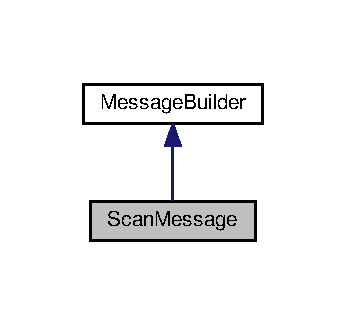
\includegraphics[width=174pt]{classScanMessage__inherit__graph}
\end{center}
\end{figure}


Collaboration diagram for Scan\+Message\+:\nopagebreak
\begin{figure}[H]
\begin{center}
\leavevmode
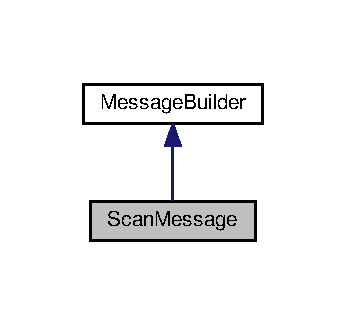
\includegraphics[width=174pt]{classScanMessage__coll__graph}
\end{center}
\end{figure}
\subsection*{Additional Inherited Members}


\subsection{Detailed Description}
This subclass generates a Scan-\/\+Message so that new Controllers on the C\+A\+N-\/\+Bus can be found. 

The documentation for this class was generated from the following files\+:\begin{DoxyCompactItemize}
\item 
/sd/triped\+\_\+app/catkin\+\_\+workspace/src/joint\+\_\+level\+\_\+control/include/joint\+\_\+level\+\_\+control/motor/message\+\_\+builder.\+h\item 
/sd/triped\+\_\+app/catkin\+\_\+workspace/src/joint\+\_\+level\+\_\+control/src/motor/scan\+\_\+message.\+cpp\end{DoxyCompactItemize}

\hypertarget{structScanResponse}{}\section{Scan\+Response Struct Reference}
\label{structScanResponse}\index{Scan\+Response@{Scan\+Response}}
\subsection*{Public Attributes}
\begin{DoxyCompactItemize}
\item 
uint16\+\_\+t {\bfseries can\+\_\+address}\hypertarget{structScanResponse_a5984426066ffa49ea49e9a1093a1f30b}{}\label{structScanResponse_a5984426066ffa49ea49e9a1093a1f30b}

\item 
uint8\+\_\+t {\bfseries mode}\hypertarget{structScanResponse_a9189a41b9ad5fc226a4c18f04399ec84}{}\label{structScanResponse_a9189a41b9ad5fc226a4c18f04399ec84}

\item 
uint32\+\_\+t {\bfseries uid}\hypertarget{structScanResponse_a03bd906c8ce581d26cf4857bf881b9cf}{}\label{structScanResponse_a03bd906c8ce581d26cf4857bf881b9cf}

\end{DoxyCompactItemize}


The documentation for this struct was generated from the following file\+:\begin{DoxyCompactItemize}
\item 
response\+\_\+messages.\+h\end{DoxyCompactItemize}

\hypertarget{classSwingJoint}{}\section{Swing\+Joint Class Reference}
\label{classSwingJoint}\index{Swing\+Joint@{Swing\+Joint}}


Inheritance diagram for Swing\+Joint\+:\nopagebreak
\begin{figure}[H]
\begin{center}
\leavevmode
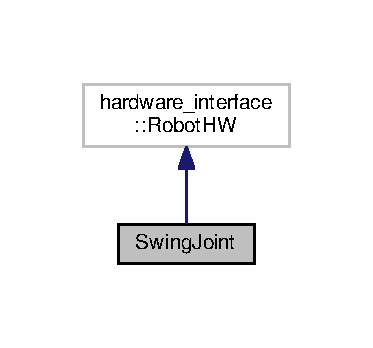
\includegraphics[width=191pt]{classSwingJoint__inherit__graph}
\end{center}
\end{figure}


Collaboration diagram for Swing\+Joint\+:\nopagebreak
\begin{figure}[H]
\begin{center}
\leavevmode
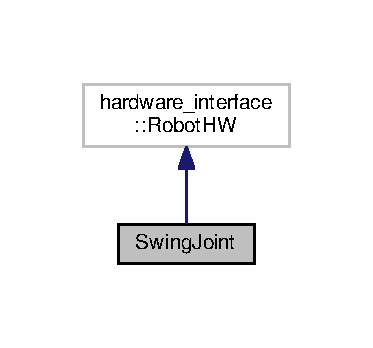
\includegraphics[width=191pt]{classSwingJoint__coll__graph}
\end{center}
\end{figure}
\subsection*{Public Member Functions}
\begin{DoxyCompactItemize}
\item 
\mbox{\Hypertarget{classSwingJoint_a283b5b0bbd8994f055995e643291b561}\label{classSwingJoint_a283b5b0bbd8994f055995e643291b561}} 
{\bfseries Swing\+Joint} (const std\+::string \&joint\+\_\+name, const std\+::string \&spi\+\_\+device, uint8\+\_\+t spi\+\_\+cs\+\_\+id, uint8\+\_\+t spi\+\_\+mode, uint8\+\_\+t spi\+\_\+bits, uint32\+\_\+t spi\+\_\+speed, uint16\+\_\+t spi\+\_\+delay, const std\+::string \&can\+\_\+name, uint8\+\_\+t can\+\_\+id)
\item 
\mbox{\Hypertarget{classSwingJoint_a3f966fc71b37d8e5c34e2ddc5ec79e03}\label{classSwingJoint_a3f966fc71b37d8e5c34e2ddc5ec79e03}} 
void {\bfseries read} ()
\item 
\mbox{\Hypertarget{classSwingJoint_aa2d54c4712616e04e36af2db528384ab}\label{classSwingJoint_aa2d54c4712616e04e36af2db528384ab}} 
void {\bfseries write} ()
\end{DoxyCompactItemize}


The documentation for this class was generated from the following files\+:\begin{DoxyCompactItemize}
\item 
/sd/triped\+\_\+app/catkin\+\_\+workspace/src/joint\+\_\+level\+\_\+control/include/joint\+\_\+level\+\_\+control/joint/swing\+\_\+joint.\+h\item 
/sd/triped\+\_\+app/catkin\+\_\+workspace/src/joint\+\_\+level\+\_\+control/src/joint/swing\+\_\+joint.\+cpp\end{DoxyCompactItemize}

%--- End generated contents ---

% Index
\backmatter
\newpage
\phantomsection
\clearemptydoublepage
\addcontentsline{toc}{chapter}{Index}
\printindex

\end{document}
